\section{Separable Similarity and Emissions}
\label{sec:separ-simil-emiss}

In the HDP-HMM-LT model, we have a defined set of states with 
locations $\ell_j$, $j = 1, \dots,
J$.  In Chapters \ref{chapter:cocktail-party} and \ref{chapter:REDD}, the similarities depended on the same parameters that determined the emission distributions, which we denoted by $\theta_j$.  In Chapter \ref{chapter:cocktail-party},
each $\theta_j$ was a binary state vector, and the similarity $\phi_{jj'}$ was a decreasing function of the distance between those state vectors, while the emission distribution was a Gaussian centered at a linear function of $\theta_j$.  In Chapter \ref{chapter:REDD}, we generalized from binary state vectors to categorical state vectors, but similarity was still based on the distance between state vectors, and emission distributions were still Gaussians centered at a linear function of the state vector.

In this chapter, we suppose instead that $\ell_{j}$ consists of two separate and a priori independent parts: $\ell_j = (\theta_{j}, \eta_{j})$, where the $\theta_j$ govern the emission distributions, and the similarities, $\phi_{jj'}$ depend on the $\eta_j$

Define
\begin{equation*}
  \phi_{jj'}(\eta_j, \eta_{j'}) = \exp\left(-\frac{\lambda}{2} \Delta_{jj'}^2\right)
\end{equation*}
where $\Delta_{jj'}$ is the Euclidean distance between $\eta_j$ and
$\eta_{j'}$; that is,
\begin{equation*}
  \Delta_{jj'}^2 = \sum_{d} (\eta_{jd} - \eta_{j'd})^2
\end{equation*}

\section{A Hamlitonian Monte Carlo step to sample $\eta$}
\label{sec:haml-monte-carlo}

Since the $\eta_j$ are real-valued vectors, we can sample them jointly using Hamiltonian Monte Carlo (HMC, also known as ``Hybrid Monte Carlo''; \citet{duane1987hybrid}, see also \citet{neal2011mcmc}).  HMC is a variation on the Metropolis-Hastings MCMC 
algorithm which is designed to more efficiently explore a high-dimensional continuous distribution by adopting a proposal distribution which is based on the evolution of Hamiltonian dynamics in a physical system.  The position of the particle in the system represents the current state of the Markov chain, the potential energy of the particle is the negative log of the target distribution, and an auxiliary ``momentum'' variable is introduced, representing the kinetic energy of the system.  The Markov chain evolves by computing a discrete approximation of an update to the position and momentum variables, and then computing the standard Metropolis-Hastings acceptance probability.

In order to carry out HMC in the context of the HaMMLeT model with latent continuous state variables given by $\eta_j$, $j = 1, \dots, J$, we need the log likelihood and log prior for the $\eta$ vector.  Assume independent and isotropic Gaussian priors on each 
$\eta_{j}$, so we have
\begin{equation*}
  p(\eta_j) \propto \exp\left(-\frac{h_\eta}{2} \sum_{d} \eta_{jd}^2 \right),
\end{equation*}
where $h_{\eta}$ is the prior precision which does not depend on $d$.

Then the log prior density, up to a constant, is
\begin{equation*}
  \log p(\eta_j) \propto -\frac{h_{\eta}}{2} \sum_{d} \eta_{jd}^2
\end{equation*}

The relevant log likelihood, as shown in Chapter \ref{chapter:HaMMLeT} is
the probability of the $z$ and $Q$ variables given the
$\phi_{jj'}$.  In particular, we have
\begin{equation*}
  L := p(\bz, \bQ \given \bphi) = \prod_{j} \prod_{j'} \phi_{jj'}^{n_{jj'}}(1 - \phi_{jj'})^{q_{jj'}}
\end{equation*}
and
\begin{equation*}
  \log L = \sum_{j} \sum_{j'} \left( n_{jj'} \log(\phi_{jj'}) +
    q_{jj'} \log(1 - \phi_{jj'})\right)
\end{equation*}

To do Hamiltonian Monte Carlo to sample from the conditional posterior
of $\eta$ given $\bz$ and $\bQ$, we need to compute the gradient of the
log posterior, which is just the sum of the gradient of the log prior
and the gradient of the log likelihood.

The $j,d$ coordinate of the gradient of the log prior is simply
\begin{equation*}
  -2h_{\eta} \eta_{jd}
\end{equation*}

To get the $j,d$ coordinate of the gradient of the log likelihood, we
can apply the chain rule to terms as is convenient.  In particular,

\begin{equation*}
  \frac{\partial L}{\partial \eta_{jd}}=\sum_{j} \sum_{j'} n_{jj'}
  \frac{\partial \log(\phi_{jj'})}{\partial \Delta_{jj'}^2}
  \frac{\partial \Delta_{jj'}^2}{\partial \eta_{jd}}+ \sum_{j}
  \sum_{j'} q_{jj'} \frac{\partial \log(1 - \phi_{jj'})}{\partial (1 -
    \phi_{jj'})}\frac{\partial (1 - \phi_{jj'})}{\partial
    \Delta_{jj'}^2} \frac{\partial \Delta_{jj'}^2}{\partial \eta_{jd}}
\end{equation*}

We have the following components:
\begin{align*}
  \frac{\partial \log(\phi_{jj'})}{\partial \Delta_{jj'}^2} &=
  -\frac{\lambda}{2} \\
  \frac{\partial \Delta_{jj'}^2}{\partial \eta_{jd}} &= 2\Delta_{jj'd} I(j \neq j')\\
  \frac{\partial \log(1 - \phi_{jj'})}{\partial (1 -
    \phi_{jj'})} &= \frac{1}{1 - \phi_{jj'}} \\
  \frac{\partial (1 - \phi_{jj'})}{\partial
    \Delta_{jj'}^2} &= \frac{\lambda}{2} \phi_{jj'}
\end{align*}
which yields
\begin{align*}
  \frac{\partial L}{\partial \eta_{jd}} &= -\lambda \sum_{j}
  \sum_{j'} n_{jj'} \Delta_{jj'd} \mathbb{I}(j \neq j') +
  \lambda \sum_{j}\sum_{j'} q_{jj'} \Delta_{jj'd} \frac{\phi_{jj'}}{1 -
    \phi_{jj'}} \mathbb{I}(j \neq j) \\
  &= - \lambda \sum_{(j,j'): j \neq j'} \Delta_{jj'd} \left(n_{jj'} - q_{jj'}
    \frac{\phi_{jj'}}{1 - \phi_{jj'}}\right)
\end{align*}
\begin{equation*}
  p(\eta_j) \propto \exp\left(-\frac{h_\eta}{2} \sum_{d} \eta_{jd}^2 \right),
\end{equation*}
where $h_{\eta}$ is the prior precision which does not depend on $d$.

\section{Synthetic Data from an HMM with a Nearly Block Diagonal Transition Matrix}
\label{sec:synthetic-data-from}


\subsection{Data-generation}

As a first check on this version of the model, several datasets were generated from fixed state Hidden Markov models whose transition matrices were close to block-diagonal.  Specifically, the state space consisted of 40 states in total which were grouped into 10 ``superstates'' of 4 states each.  With probability 0.95, the chain transitioned to another state in the same superstate, and with probability 0.05 it transitioned to a different superstate.  The distribution across the 4 same-superstate entries was drawn for each row from a symmetric Dirichlet, where the concentration parameter varied across datasets.  The distribution for each row across the 8 other-superstate entries was drawn from a symmetric Dirichlet as well, where again, the concentration parameter was varied.

Each of the forty states was associated with a mean in a two-dimensional observation space.  However, unlike in the experiments discussed in Chapters \ref{chapter:cocktail-party} and \ref{chapter:REDD}, there was no relationship between proximity in transition space and proximity in emission space: the means for the twelve states were drawn independently from a $\Norm{0}{\sigma^2 I}$ distribution, where $\sigma^2$ was varied across datasets.

At each time step, an observation was drawn from a bivariate $\Norm{\mu_j}{I}$ distribution.

Since the HaMMLeT model infers a latent location for each state, and since the latent state locations impact the transition matrix by promoting transitions between nearby states and suppressing transitions between far away states, it is predicted that the HaMMLeT model will locate states in the same superstate near each other, and so we should expect to see a ``clustering'' of states into three distinct groups based on their $\eta_j$ vectors.  This clustering ability should allow HaMMLeT to more efficiently learn the correct transition matrix as compared to the HDP-HMM with no preference for local transitions.

To evaluate the performance of HaMMLeT versus the ordinary HDP-HMM, each models' calculated marginal log likelihood was computed based on both the training data set used during inference, and on a held-out test set.  At each Gibbs iteration, the marginal log likelihood was computed by fixing the transition matrix and emission parameters, and integrating out the state sequence using the forward message passing algorithm.

\subsection{Results}

\begin{figure}
\begin{minipage}{0.45\textwidth}
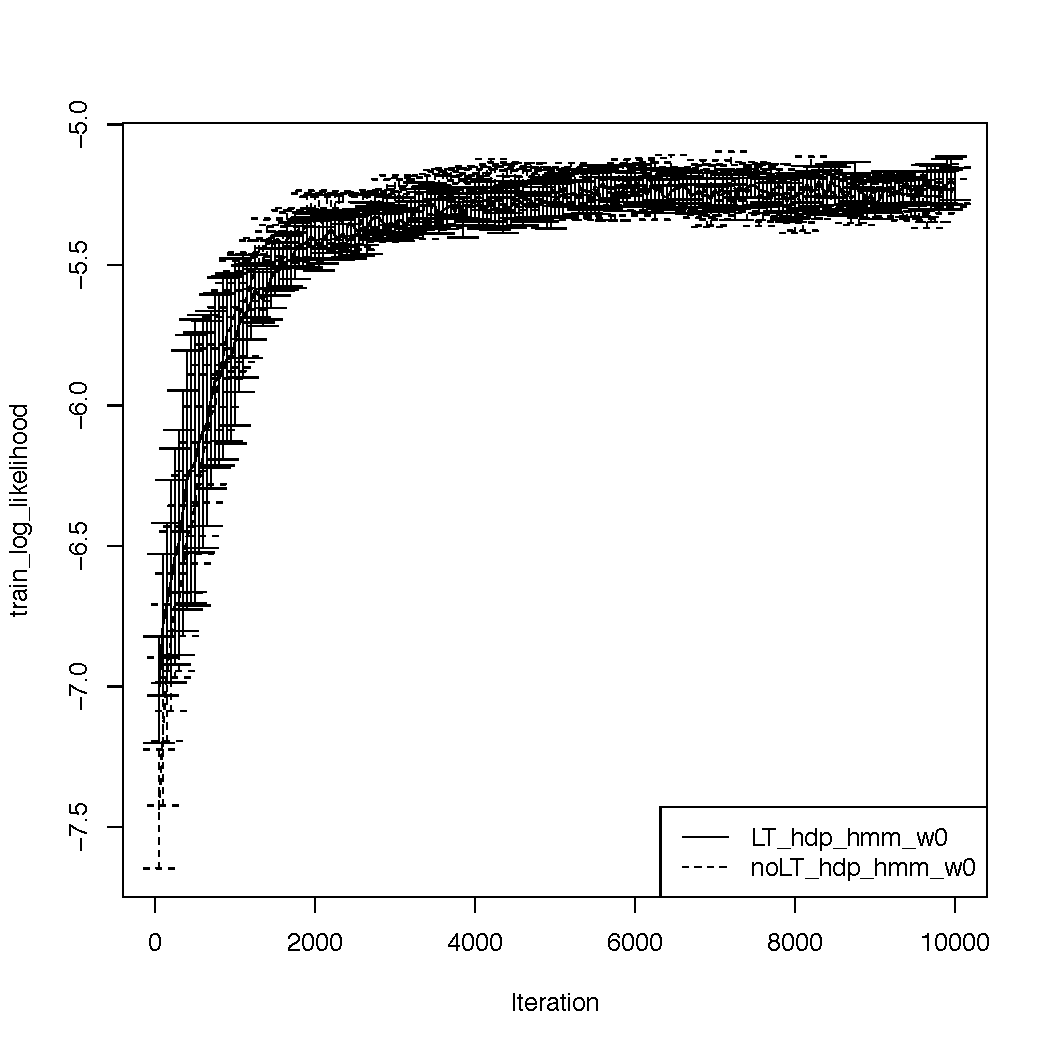
\includegraphics[width=\textwidth]{fig/block_diag/train_log_likelihood}
\end{minipage}
\hspace{0.1in}
\begin{minipage}{0.45\textwidth}
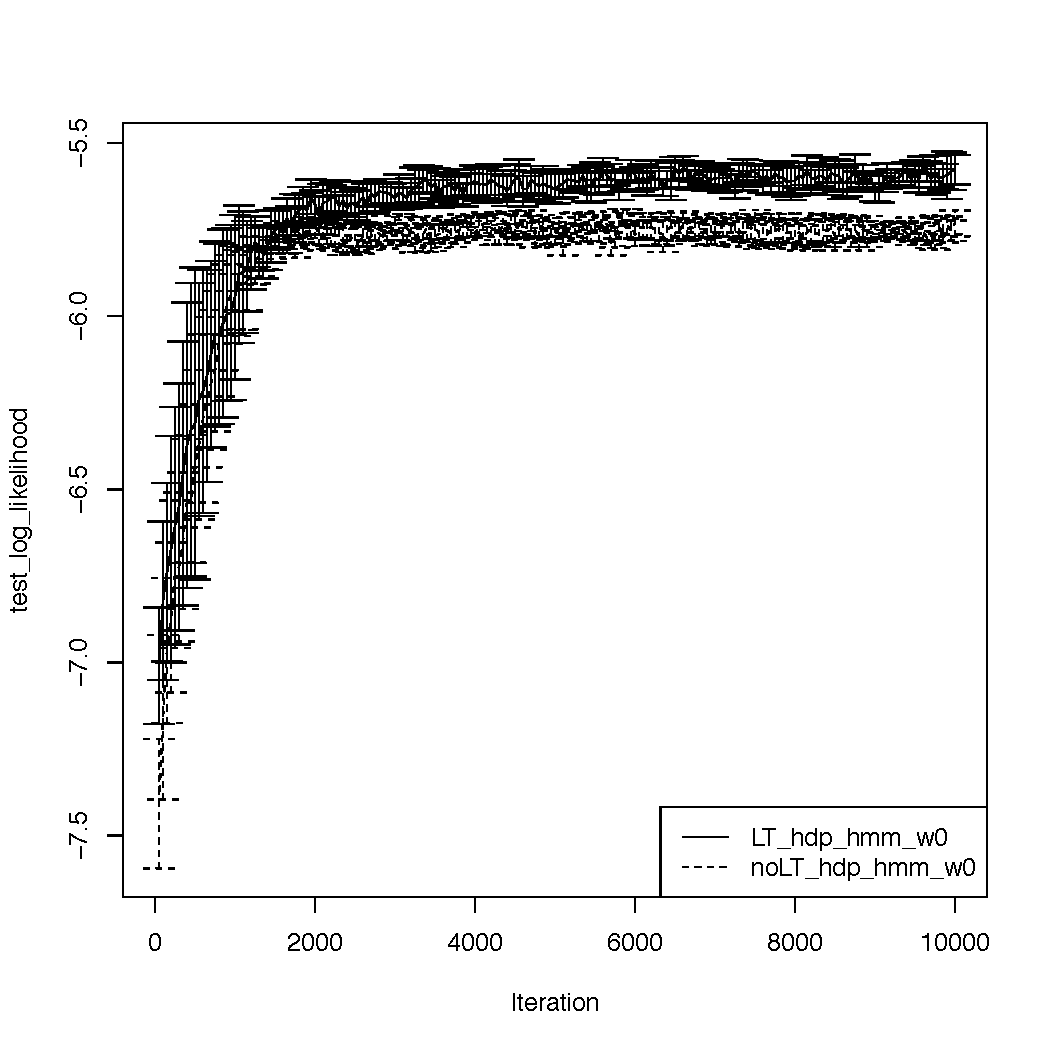
\includegraphics[width=\textwidth]{fig/block_diag/test_log_likelihood}
\end{minipage}
\caption{Left: Log likelihood on the training set by Gibbs iteration
  (marginalizing out state sequence) for LT and no LT (HDP-HMM)
  models.  Right: Log likelihood on a held out test set.}
\end{figure}

\section{Discovering Chord Equivalence Classes in Tonal Music}
\label{sec:disc-chord-equiv}

A real-world test of the separable-similarity form of HaMMLeT comes from the music domain.  We employed a dataset in which each observation consisted of four musical tones played concurrently, constituting a chord, and where the sequences between chords followed conventions for Western tonal music. 